\subsection{Overview}
Our system is designed in a client/server way, where clients send job
requests to the server using a simple customized language, which
specifies things such as which application to use, which input files
to use, etc., and the server parses the requests, creates a
corresponding job and then put it into the pending job queue. The job
is then waiting for dispatch by the scheduler.

\begin{figure}[!t]
\centering
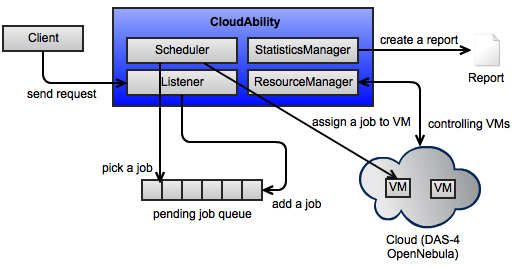
\includegraphics[width=0.35\textwidth]{pictures/system-arch.png}
\caption{CloudAbility Architecture Overview}
\label{figure_system_arch}
\end{figure}

The server part of the system consists of the following components:

\begin{enumerate}
\item\emph{Listener}:
The listener is responsible for accepting client requests through
socket connection, parsing them, and put the jobs into the pending job
queue.
\item\emph{Scheduler}:
The scheduler is the core thread in the system. It does scheduling
according to the given allocation and provisioning policies and
updates current system status. It will be explained in more details in
the later part.
\item\emph{ResourceManager}: 
This component manages the VM instances on the cloud. It also holds the
provisioning policy and provides a public interface to use it.
\item\emph{StatisticsManager} 
This module maintains all the statistics data of the system, including
job performances, VM instance performances, etc. It also generates a
final report when the system is shutting down.
\end{enumerate}

Our system is currently only runnable on \textsc{das-4} OpenNebula
platform, but it can be easily modified and extended to support other
cloud platforms. It is easy to create new allocation and provisioning
policies. All configurations are done through a configuration file.


\subsection{Resource Management Architecture}
Some features must be explained before we go to more details.

\subsubsection{Jobs}
There are three job queues in the system: \emph{pending job queue},
\emph{running job queue}, and \emph{finished job queue}. A pending job
will be picked by the scheduler and assigned to a VM instance. Then a
thread for executing this job is created, and the execution is done in
the following sequence:

\begin{enumerate}
\item Downloading required files (in our case, executable tarball and
  input files).
\item Extracting the executable tarball.
\item Executing the job (converting H.264 video file into
  \textsc{ntsc-dvd}).
\item Uploading the resulting \textsc{dvd} file to the server.
\end{enumerate}

All these operations are done through \textsc{scp} and \textsc{ssh}.
The job thread is also responsible for collecting its performance
statistics, including downloading time, execution time, uploading
time, etc. Once this job is done, it will be put into the
\emph{finished job queue} with its state set to \statefinished. Later,
the scheduler will remove this job and update the statistics. If a job
fails, it will also be put into the \emph{finished job queue} but with
its state set to \statefailed.  The scheduler will handle these failed
jobs according to the given policy.

Although the parameters---which specifies which application to run, which
files to download, etc.---are configurable to make it able to do other
tasks, our design is not that flexible because this execution sequence
is hard coded in the program. We will consider using script files for job
execution.


\subsubsection{VM instances}
In OpenNebula, after a VM instance is created, its state becomes
\statepending and you need to wait until it is \staterunning.
At this point, the VM instance is running, but it may not be actually
\emph{ready} because when it becomes \staterunning, it still needs some
time to boot the OS and initialize the system. Only after the system is
fully booted can the VM instance be accessed using \textsc{ssh}.

In our system, a VM instance is created asynchronously: a
thread called ``VMAgent'' is created every time the system creates a
VM instance. This thread first allocates the VM instance and then
does the following things:

\begin{enumerate}
\item It waits until this VM instance becomes \staterunning.
\item It waits until the VM can be reached by ping.
\item It waits until the VM can be reached by \textsc{ssh}.
\end{enumerate}

After the VM is reachable, it is added into the VM list in the
ResourceManager and it becomes available for jobs to execute on.

Each VMAgent has a timeout of two minutes. If the operation times out,
the VM instance will be terminated.

\subsubsection{Scheduler}
What the scheduler does is as follows:

\begin{enumerate}
\item It does some regular checks and updates, which will be explained
  later.
\item It picks a job from the \emph{pending queue} using the specified
  job allocation policy.
\item It picks a VM instance using the specified resource provisioning
  policy.
\item It executes this job on this VM instance.
\end{enumerate}

In the regular check part, the scheduler does miscellaneous tasks,
including:
\begin{itemize}
\item Updating job states, VM instance states and system states.
\item Checking the \emph{finished job queue}. If a job is finished
  successfully, it is removed and its data is used to update the
  statistics. If it failed, it will be handled according to the given
  job allocation policy. For now, the system just puts a failed job into
  the \emph{pending job queue} again regardless of how many times it
  has failed.
\item Calling the provisioning policy to perform elastic provisioning.
\end{itemize}

In this way, the statistics of the system is continuously recorded
and flexible allocation policies and elastic provisioning policies can
be implemented.


\subsubsection{Reliability}
Our system keeps track of every job and VM instance. During the
shutdown sequence, it first stops all executing jobs. Then, it
terminates all allocated VM instances, so that no VM instance would be
running afterwards. After that, it checks jobs in all the queues and
put them into the statistics module, which finally creates a report
and outputs to a file.

Besides that, our system also keeps separate log files for the system
itself and each jobs respectively.


\subsection{System Policies}
We have implemented one job allocation policy and two resource
provisioning policies.

\subsubsection{Allocation Policy}
The job allocation policy we implemented is a First-Come-First-Serve
(\textsc{fcfs}) policy. It always picks the pending job with the
earliest arrival time.

\subsubsection{Provisioning Policies}
We implemented two provisioning policies: \policystatic{} policy and
\policysimpleelastic{} policy.

The \policystatic{} policy allocates a fixed number of VM instances when the
system starts and this number will not vary over time. This policy
can not adapt itself to the changing environment.

The \policysimpleelastic{} policy is an on-demand-like elastic policy, which has
three parameters:

\begin{itemize}
\item \emph{min-vms}: The minimum number of VM instances the system
  must have.
\item \emph{max-vms}: The maximum number of VM instances the system can
  have.
\item \emph{threshold}: A threshold value, which will be explained
  later.
\end{itemize}

Each time the system statuses have been updated by the scheduler, this
provisioner is called and it checks the number of pending jobs. If
this number is larger than the \emph{threshold}, it creates one more
VM instance until either (1) the total number of VM instances in the
system equals the sum of pending jobs and running jobs or (2) it reaches
the \emph{maxvms}. However, when the pending job queue becomes empty,
this policy will find one idle VM instance and release it.

The \policysimpleelastic{} policy is a simple on-demand policy is because
it doesn't take into account how long a VM instance has been idle. It simply
terminates one if it is currently idle. A main drawback of this policy
can be illustrated in this example: suppose there are 7 jobs running,
no pending jobs and 8 VMs in the system. So this policy will remove
one idle VM. If a job arrives right after the policy removes a VM,
this job has to wait for a long time to obtain an available VM.

\subsection{Implementation}
Our implementation is done in Java and the following libraries are
being used:

\begin{itemize}
\item Apache \textsc{xml-rpc}\cite{URL:ApacheXmlRpc} for implementing the module
  that interacts with OpenNebula through its \textsc{xml-rpc} API.
\item We used trilead-ssh2\cite{URL:trilead-ssh2} to establish
  \textsc{ssh} and \textsc{scp} connections with the VMs.
\item Apache log4j\cite{URL:ApacheLog4j} is used for system logging.
\end{itemize}
